% Name: Bisecting an angle with compass and straightedge
% Description: An arc about O cuts the arms at P and Q, equal arcs about P and Q cross at R, and the ray OR bisects the angle.
% Tags: construction, angle bisector, compass and straightedge, ruler and compass

\usetikzlibrary{angles, quotes}

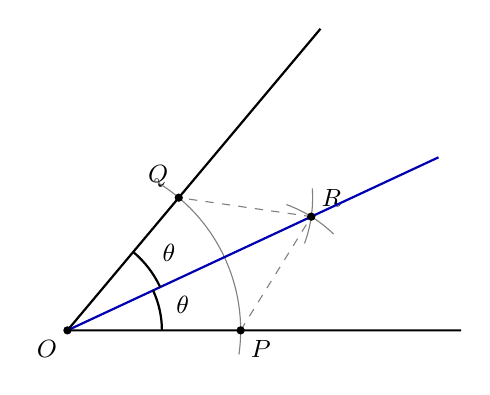
\begin{tikzpicture}[thick, every node/.style={font=\small}]
  % Angle 50 degrees, first arc radius 2.2, second arcs radius 1.7: R = 3.4171 along 25 degrees; RP points at 58.16 degrees and RQ at -8.16 degrees
  \coordinate[label=below left:$O$] (O) at (0,0);
  \coordinate (X) at (5,0);
  \coordinate (Y) at (50:5);
  \coordinate[label=below right:$P$] (P) at (2.2,0);
  \coordinate[label=above left:$Q$] (Q) at (50:2.2);
  \coordinate[label=above right:$R$] (R) at (25:3.4171);
  \draw (X) -- (O) -- (Y);
  \draw[gray, thin] (-8:2.2) arc[start angle=-8, end angle=60, radius=2.2];
  \draw[gray, thin] (P) ++(46:1.7) arc[start angle=46, end angle=70, radius=1.7];
  \draw[gray, thin] (Q) ++(-20:1.7) arc[start angle=-20, end angle=4, radius=1.7];
  \draw[dashed, gray, thin] (P) -- (R) -- (Q);
  \draw[blue!70!black] (O) -- (25:5.2);
  \pic[draw, angle radius=12mm, "$\theta$", angle eccentricity=1.25] {angle=X--O--R};
  \pic[draw, angle radius=13mm, "$\theta$", angle eccentricity=1.25] {angle=R--O--Y};
  \foreach \p in {O, P, Q, R} \fill (\p) circle (1.5pt);
\end{tikzpicture}
